% show my problem is unsolved
% • show my problem is interesting
% • show my idea works
% • show how my idea compares to other ideas
% • No related work yet! Include at end.
% – Problem 1: describing alternative approaches gets between the reader
% and your idea (I feel tired)
% – Problem 2: the reader knows nothing about the problem yet; so your
% (carefully trimmed) description of various technical tradeoffs is abso-
% lutely incomprehensible (I feel stupid)
% – instead, Concentrate single-mindedly on a narrative that
% ∗ Describes the problem, and why it is interesting
% ∗ Describes your idea
% ∗ Defends your idea, showing how it solves the problem, and filling
% out the details
% ∗ On the way, cite relevant work in passing, but defer discussion to
% the end
% • show how my idea compares to other ideas
% • Be generous to the competition. In his inspiring paper [Foo98] Foogle shows....
% We develop his foundation in the following ways...
% • Giving credit to others does not diminish the credit you get from your paper
% • Acknowledge weaknesses in your approach
% • Failing to give credit to others can kill your paper: You don’t know that it’s
% an old idea (bad) or You do know, but are pretending it’s yours (very bad)
% ===================================================
\chapter{Background}
\label{ch:background}
% ===================================================

% ===================================================
\section{Parking Spot Placement for Autonomous Wheelchairs}
% ===================================================
% Purpose: Motivate the need of an autonomous back-in parking system.

With the number of US citizens over the age of 65 expected to grow by 75\% by
2030 \cite{simpson2008many}, ensuring older adults maintain their sense of
mobility becomes increasingly important.
For residents in long-term care facilities, independent mobility is directly
related to their quality of life and sense of freedom, choice and independence
\cite{bourret2002meaning}.
For people of any age, loss of independent mobilitiy leads to feelings of
emotional loss, reduced-self esteem, isolation, stress and fear of abandonment
\cite{finlayson2003experiencing}, and decreases opportunities to socialize that
lead to anxiety and depression \cite{iezzoni2001mobility}. 

Wheelchairs offer a solution, but many users find operating existing manual or
powered wheelchairs (PWCs) difficult or impossible \cite{simpson2008many}.
10\% of patients who receive PWC training find it extremely difficult or
impossible to use the wheelchair for activities of daily living, and
when asked specifically about steering and maneuvering tasks, the
percentage jumps to 40\% \cite{fehr2000adequacy}.
Fehr et al. \cite{fehr2000adequacy} concludes improving steering interfaces is
not enough due to the type of impairments the users face, and autonomous
navigation is necessary. Half of patients unable to normally control a powered
wheelchair would benefit from an automated navigation system.
This population that stands to benefit is significant:
In 2008, 1.4 to 2.3 million people in the US were estimated to
benefit from powered wheelchairs with some autonomous functions, and of those
973,000 to 1.7 million will benefit particularly from autonomous
navigation capabilities with a growth rate of 5.9\% per year \cite{simpson2008many}.
Powered wheelchairs (PWCs) with autonomous maneuvering capabilities are both
necessary and will directly improve the quality of life of millions of people.

Complete PWC automation, however, is not suitable. 
A totally autonomous system may deprive a user's feeling of being in control 
\cite{viswanathana2014wizard}.
Older adults preferred robot assistance over human assistance for tasks related
to chores, manipulating objects, and information management, but not personal
care and leisure activities \cite{smarr2014domestic}.
Instead, task-specific autonomous routines is preferable, akin to automatic
parallel parking or cruise control in a car.
Some work has been done on task-specific autonomous PWC behaviours, including
navigation in crowded environments \cite{prassler2001robotics}, obstacle
avoidance \cite{viswanathan2012navigation}, and docking onto lift platforms
\cite{sermeno2006vision} and custom-designed beds \cite{ren2012docking}.
More general overviews of smart wheelchair systems have also been described
\cite{viswanathan2012navigation, simpson2005smart, faria2013patient}. 

One common task is back-in parking [TODO bikram thesis/pooja's draft]. 
% Not much in general back-in parking, a very common task in the target demographic
Little work has been done to dock/back-in park a wheelchair in a more general
environment, such as an indoor office or a room in a long-term care facility. 

This motivates the application of the work in this thesis:
we focus on automating the back-in parking task for a PWC, a specific task that
has been proven desirable and helpful to be automated.


\begin{figure}
\centering
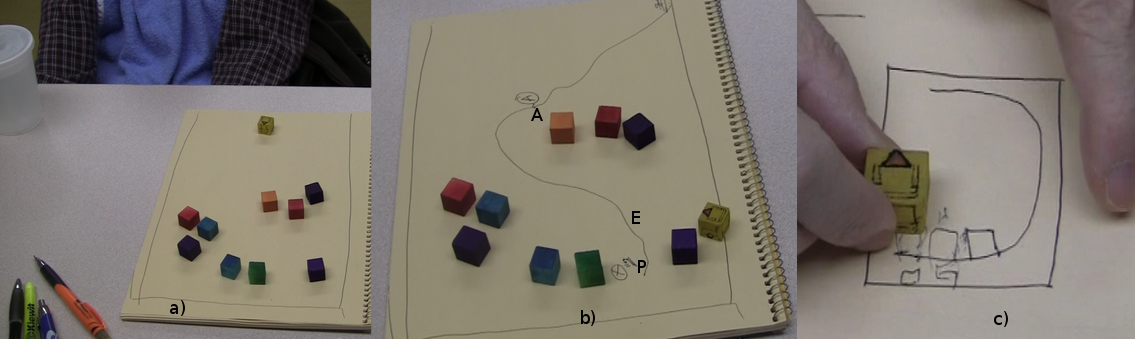
\includegraphics[width=5in]{figures/bikramjoe.png}
\caption{From \cite{adhikari2014single}. A user study simulating a sing-along
gathering scenario. a) shows an initial wheelchair configurations (represented as
blocks) with the user controlling the yellow block. b) shows the suggested
trajectory by the user. c) shows how the user characterizes parking spots in an
open space.}
\label{fig:bikramjoe}
\end{figure}

% \section{Motion Planning with Ill-Defined Goal States}
% 
% Lots of work has been done to determine a path given a goal state/set. This
% assumes a goal set has been previously defined.
% 
% Lots of work has been done on determining objects, scenes. But little work has
% been done to combine the two: Determinine a suitable goal state that takes into
% account feasibility and choosing a goal state that is present in the scene. 
% 
% This is closely related to developing a potential function: a pseudo-metric that
% defines how close you are to a goal. Our work skips the 'given a goal state,
% design a potential function' step, and develops a potential field as a
% by-product of generating goal states.
% 
% Often it makes sense to have a fixed goal set, or one goal state. If your robot
% wants to reach the fridge, having the location of the fridge is an appropriate
% goal.
% We do away with the notion that there is a fixed goal set. Often the goal set is
% fuzzy, we do not know much about it. Instead, we form a desirability function
% (which can be seen as a negative potential field) over the configuration space.
% We then plan to reach a high level in the desirability function given certain
% constraints.
% 
% Take, for example, the problem of placing a robot to rest for a night. Where
% should you place it? In most cases there isn't a correct answer. There is no
% well-defined goal state. There are also constraints that must be satisfied:
% obstacle avoidance, minimum path length. Instead of posing the problem as path
% planning towards an arbitrary goal state, we pose it as steering the robot to an
% incrementally better configuration.
% 
% It's often assumed you can see what your goal state is like. There are a lot of
% times a goal state isn't defined by what it looks like, but by the context
% surrounding it: perhaps it is an enclosed space that fits the robot just right.

% ====================
\subsection{Problem formulation}
% ====================
We address the problem of determining a parking spot for a wheelchair.
Specifically, we are concerned with identifying where in a room should a
wheelchair be placed that minimizes inconvenience and obstructions and best
coincides with human preference.

[TODO figure]
Let us start with examples to illustrate the problem and some desirable
properties.
Figure X shows an example floor plan, with various objects of different sizes
and locations: other wheelchairs, tables, chairs and cabinets. We would like to
find location to place the wheelchair, in green.  Figure A shows one scenario:
we would prefer placing the wheelchair in a corner out of the way, rather than
in the middle of an open floor which may obstruct people's movements.  In group
gatherings at long-term care facilities, wheelchairs tend to be packed along the
sides of a room.
Figure B
shows another: we would like to place the wheelchair to allow for a additional
wheelchairs to be placed beside it. This makes more efficient use of space.
Figure C shows that we would like to place wheelchairs only in places that can
be reached, and to find a parking spot with orientations aligned with walls, to
also make the most of the given space.

We start with the following assumptions:
\begin{itemize}
\item Objects in the room are typical to indoor office environments. These
include but are not limited to: chairs, other wheelchairs, tables and cabinets.
\item Objects will be static/non-moving
\item The floor will be flat throughout (i.e. no ramps)
\item The user will have pre-moved their wheelchair to direct the camera to the
general area of where they wish to park. This avoids dealing with shared control
directly; the user's intentions are given a priori through the current
wheelchair position.
\item Subsequently, a parking spot is entirely in view of the sensor, with no
objects obstructing any part of the parking spot. This assumption may not hold
for parking spots in tight corners.
\end{itemize}


\subsection{Characteristics of a good parking spot}
\begin{itemize}
\item Minimize 'useless' space, space that another wheelchair cannot fit in 
\item minimize tight spaces, holes, blockades
\item be parallel/perpendicular to walls
\item must be reachable from the current location in a reasonable amount of
time: one smooth motion instead of many iterations of forward/reversing
\item related: takes into account non-holonomic constraints
\item maximize usable free space, minimize wasted space
\item maximize the amount of contiguous space: space that is wide open is more
desirable
\item ensure wheelchair's 'safety': a margin of error, the parking spot
shouldn't be directly touching any objects
\end{itemize}

We return to these characteristics during evaluation in section [TODO], where we
develop quantatitive measures.

% ====================
\section{Parking Lot Detection}
% ====================
% Wang \cite{wang2014automatic}
% Jung \cite{jung2014semiautomatic}
% 
% Pouria's thesis \cite{talebifard2014risk}
% Talk: \url{https://www.youtube.com/watch?v=Db7EhLYf-Yk#t=1h11m07s}
% 
% 
% file:papers/jiang1999sensor.pdf
% Basic old paper on parallel parking. Uses ultrasonic sensor, then
% fixed planning.
% 
% file:papers/fairus2011development.pdf
% Old paper. Scanning methods.
% 
% file:papers/wang2013automatic.pdf
% Newish lit review of automatic parking
% 
% file:papers/abad2007parking.pdf
% Parking space detection using 3d vision. Parallel parking
% 
% file:papers/lalonde2012single.pdf
% CVPR workshop paper.
% 
% file:papers/suhr2010automatic.pdf
% Good! Solving my problem, but with a laser rangefinder.
% found from: http://www.mathworks.com/matlabcentral/answers/126413-how-to-detect-free-spots-in-a-parking-area
% 
% file:assets/WheelchairGuide.pdf
% ====================
\section{Related Work}
\label{sec:parkinglotidentificationlitreview}
% ====================
Detecting a parking spot poses an interesting problem. Unlike a standard object
detection pipeline, a parking spot is not determined by the appearance of an
object, but by the presence of negative space within an area. The context of the
scene also determines where an adequete parking spot should be. In this way, an
ideal parking spot is not purely identifiable by the features within it; but
instead is determined by contextual cues surrounding it.


\subsection{Outdoor Parking Lot Detection}

Many methods formulate the problem of identifying a parking spot
as a detection problem, where a parking spot is to be detected within the scene
using supervised classification techniques.

Work has been done to determine locations of parking spots for cars in car lots
[citations]. 
\cite{wu2006parking, true2007vacant}

Suhr \cite{suhr2010automatic} detects parking spaces in a similar way to ours.
They detect parking spaces by first detecting neighbouring cars using geometric
constraints. Our method, in contrast, does not require such hardcoded
constraints.


Many of these techniques rely on the presence of parking spot
lines, and use line detection algorithms to do so. Once the parking spot is
found, a support vector machine is trained on empty and occupied parking spots.

These methods rely on accurate identification based on line markings, which are
not present in indoor environments not purely dedicated to parking. 

Formulating the problem as a classification problem is then harder, as
classification must be done on any feasible area instead of just a set number of
pre-identified parking spots.

These algorithms also do not address which of the found parking spots to choose:
in a car parking lot, one spot dominates the camera due to the close proximity
of the car to the spots. However, in an indoor wheelchair environment, many
parking lots exists.

TODO researchlog/thesis.org for references.

Many techniques using location-tailored hardware to detect free parking spaces
in car parking lots, involving wireless sensors \cite{panja2011wirelessly},
pre-existing security cameras \cite{true2007vacant} and magnetic field detectors
\cite{boda2007design}. In contrast, our method aims to detect free parking
spaces with only sensors onboard the wheelchair: no external sensors and even no
external pre-determined parking lot spots.


\subsection{Packing Problems}
This problem also has similarities to packing problems \cite{dyckhoff1990typology}.

The general packing
problem tries to, given a set of rectangular objects, pack as many as possible
in a larger rectanle. In our case, we are given one wheelchair, and we may wish
to pack it in a space that is least obstrusive to other areas.

Pallet loading problem \cite{martins2008solving}:
Pallet Loading Problem (PLP). PLP max- imizes the number of boxes placed on a
rectangular pallet. All boxes have identical rectangular dimensions and, when
placed, must be located completely within the pallet. Boxes may be rotated 90°
so long as they are placed with edges par- allel to the pallet’s edges. The set
of all PLP instances with an area ratio (pallet area divided by box area) less
than 101 boxes can be represented by 3,080,730 equivalent classes.


TODO researchlog/thesis.org for references.


% *** Packing Problems
% This is a problem in operations research.
% 
% http://en.wikipedia.org/wiki/Packing_problems
% http://www.codeproject.com/Articles/210979/Fast-optimizing-rectangle-packing-algorithm-for-bu
% Problem: In the visible ground, pack as many wheelchairs as possible in it, and then find the best position
% - pack as densely as possible: maximize 'walkable space': space connected to free space
% - constraints: each wheelchair must be able to reach the parking spot
% 
% "Computational Packing Problem"
% http://scholar.google.ca/scholar?q=computational+packing+problem&hl=en&as_sdt=0&as_vis=1&oi=scholart&sa=X&ei=DYxKVeqHHdCNoQT684Eg&ved=0CBsQgQMwAA
% 
% file:papers/hopper2000empirical.pdf
% file:papers/martello2000three.pdf
% 
% Looks like state-of-art:
% http://www.ijcai.org/papers09/Papers/IJCAI09-092.pdf
% 
% I can frame my problem as such:
% - Packing problem, rectangles in arbirtary container
% - with additional constraint of feasability to go from current configuration to target configuration
% 
% *** Tetris Problems
% https://luckytoilet.wordpress.com/2011/05/27/coding-a-tetris-ai-using-a-genetic-algorithm/
% - penalize holes
% - penalize blockades
% 
% **** Tetris is hard, even if the sequence is known
% http://en.wikipedia.org/wiki/Tetris#Computational_complexity


\subsection{Choosing the best parking spot}
\cite{bogoslavskyi2015where} identifies where best to park using an MDP?.

This addresses the issue of how best to choose a parking spot given multiple
candidates. However, it does not work over continuous space, which is what we
have.

\subsection{Choosing the best parking spot, game-theoretic approaches}
Given locations of free car parking spots in a city, Ayala et al.
\cite{ayala2011parking} attempts to choose the ideal parking spot location
in a game-theoretic framework. TODO READ.
\cite{ayala2012parking}

\cite{mejri2014cooperation} uses performance metrics: average distance between
the vehicle and assigned slot, and others.

\cite{alfonsetti2014semi} states: 
As a result, almost all existing methods for parking slot assignment are simple
and greedy approaches, where each car is assigned a free parking slot, which is
closer to its destination. Moreover, no emphasis is placed to optimize the
social benefit of the users during the parking slot assignment. 

\subsection{Path planning with ill-defined goal states}
"Path Planning on Grid Maps with Unknown Goal Poses"

Quote from \cite{javdani2015shared}:
Maximum  entropy  inverse  optimal  control  (MaxEnt  IOC)
methods  have  been  shown  to  be  effective  for  goal  predic-
tion [28, 29, 30, 7]

Quote from \cite{javdani2015shared}:
Others have approached the prediction problem by utilizing
various machine learning methods. Koppula and Saxena [15]
extend  conditional  random  fields  (CRFs)  with  object  affor-
dances  to  predict  potential  human  motions.  Wang  et  al.  [23]
learn  a  generative  predictor  by  extending  Gaussian  Process
Dynamical Models (GPDMs) with a latent variable for inten-
tion. Hauser [11] utilizes a Gaussian mixture model over task
types  (e.g.  reach,  grasp),  and  predicts  both  the  task  type  and
continuous  parameters  for  that  type  (e.g.  movements)  using
Gaussian mixture autoregression.

\subsection{Shared Control}
Hindsight optimization to choose and move between goal states
\cite{javdani2015shared}.

Quote from \cite{javdani2015shared}:
Recently,  Hauser  presented  a  system  which  provides
assistance  while  reasoning  about  the  entire  distribution  over
goals.  Given  the  current  distribution,  the  planner  optimizes
for  a  trajectory  that  minimizes  the  expected  cost,  assuming
that no further information will be gained. After executing the
plan for some time, the distribution is updated by the predictor,
and a new plan is generated for the new distribution. In order
to  efficiently  compute  the  trajectory,  it  is  assumed  that  the
cost function corresponds to squared distance, resulting in the
calculation decomposing over goals. In contrast, our model is
more  general,  enabling  any  cost  function  for  which  a  value
function  can  be  computed.  Furthermore,  our  POMDP  model
enables us to reason about future human actions.  \cite{hauser2013recognition}
% ====================
\section{Packing Problems}
% ====================
% ====================
\section{Goal State Inference}
% ====================
% ===================================================
\section{Notation for Traditional Path Planning}
% ===================================================

[TODO avoid definition notation]
\theoremstyle{definition}
\begin{definition}{Maximal Reachable Set}
A fibration is a mapping between two topological spaces that has the homotopy lifting property for every space $X$.
\end{definition}

Taken from page 17 of \cite{lavalle2006planning}:


page 29, formulation 2.1 of \cite{lavalle2006planning}:
\subsection{Discrete Feasible Planning}
\begin{description}
  \item[State Space] non-empty state space X. In our case, we have
  $SE(2)$ (TODO Check), $(x,y,\theta)$
  \item[Initial State] a state in $X$
  \item[Goal Set] a subset of $X$
  \item[Action Space] The second item
  \item[State Transition Function] The third etc \ldots
\end{description}

% ======================
\endinput
Any text after an \endinput is ignored.
% ======================
% ====================
\section{SLAM}
% ====================

LSD-Slam and PTAM for monocular seem to be state-of-art: \url{http://vision.in.tum.de/research/lsdslam}

review paper: \url{http://www-personal.acfr.usyd.edu.au/tbailey/papers/slamtute2.pdf}

2009 review paper: \url{http://www.le2i.cnrs.fr/IMG/publications/2172_Muhammad_EI_2009.pdf}

We avoid the use of a global map. In long-term care environments, tables,
chairs, parked wheelchairs, and other objects are frequently moved around,
requiring consistently updating sensing. Instead, we use a local map in a tight
feedback loop. We treat each frame independently. This memoryless pipeline has
many desirable properties: it inherently adapts to quick changes and can be
stopped and started anytime.

% ====================
\section{Collision Avoidance}
% ====================
Old paper using quadtrees\cite{ghoshray1996comprehensive}

Bigdog \cite{raibert2008bigdog}

Springer handbook of robotics \cite{siciliano2008springer}: Vector field histograms, as described in Pouria's thesis \cite{talebifard2014risk}


% ====================
\section{Time Optimal Trajectory Planning}
% ====================
\cite{fiorini1996time}

% ===================================================
\section{Robotics Pipelines}
% ===================================================

% ---------------------------------------------------
\subsection{Robotic Operating System}
% ---------------------------------------------------

% ---------------------------------------------------
\subsection{Robotic Operating System}
% ---------------------------------------------------

% ===================================================
\section{Modeling}
% ===================================================

% ---------------------------------------------------
\subsection{Classification}
% ---------------------------------------------------
Modeling 

% ---------------------------------------------------
\subsection{Bayesian Stuff}
% ---------------------------------------------------
Chiu-Liu Trees

% ---------------------------------------------------
\subsection{Markov Chains, MDPs, POMDPs}
% ---------------------------------------------------

% ---------------------------------------------------
\subsection{Reinforcement Learning}
% ---------------------------------------------------
Value function, reward function

% ---------------------------------------------------
\subsection{Path Planning}
% ---------------------------------------------------

% ---------------------------------------------------
\subsection{Bandit Problems}
% ---------------------------------------------------

% ---------------------------------------------------
\subsection{Feasibility}
% ---------------------------------------------------

% ---------------------------------------------------
\subsection{Game Theory}
% ---------------------------------------------------

% ---------------------------------------------------
\subsection{Control}
% ---------------------------------------------------

% ---------------------------------------------------
\subsection{Rotations}
% ---------------------------------------------------

% ---------------------------------------------------
\subsection{Distance Transforms and Geodesics}
% ---------------------------------------------------

% ---------------------------------------------------
\subsection{Visual Servoing}
% ---------------------------------------------------
% https://en.wikipedia.org/wiki/Visual_servoing
